\section{안정성 분석}\label{sec:stability}
아래 진술은 비포화·무잡음 선형 폐루프에 관한 것이며 포화 비선형 시뮬레이션으로 자동 확장되지 않는다.

LQR의 불확실 스칼라 특성방정식은
\begin{equation}
z-[A_d(C_{\rm th},UA)-B_d(C_{\rm th},UA)K]=0 \label{eq:lqrchar}
\end{equation}
이다. 연속 상자 $C_{\rm th}\in[0.7,1.3]C_0$, $UA\in[0.7,1.3]UA_0$에서 단조 지수 경계로 $A_d$와 $B_d$의 구간을 구한다. \cref{eq:lqrchar}의 자연 구간 평가는 단위원 여유 0.003961을 남겨 이 상자에서 기존 LQR을 형식적으로 인증한다.

LQI 폐루프 행렬은
\begin{equation}
F_{\rm LQI}=\begin{bmatrix}A_d-B_dK_x&-B_dK_z\\-h&1\end{bmatrix} \label{eq:lqimatrix}
\end{equation}
이다. 특성다항식 $z^2-tz+\delta$의 2차 Jury 조건은 $1-t+\delta>0$, $1+t+\delta>0$, $1-\delta>0$이다. $128^2$개의 덮개 부분 상자에서 바깥쪽으로 보수적인 구간 평가를 수행한 최소 여유는 각각 $3.19\times10^{-5}$, 3.95, 0.0137이다. 모두 양수이므로 연속 상자 전체에서 기존 LQI 안정성이 인증된다. 세분화는 의존성 과대평가만 줄이며 점을 누락하지 않는다.

구현된 PID는 적분 상태, 필터 미분 상태, 이전 측정값 때문에 4차 선형 실현을 갖는다. 특성방정식은 $\det(zI-F_{\rm PID})=0$이며 $F_{\rm PID}$는 이산 갱신식에서 직접 생성한다. 61×61 격자의 스펙트럼 반경은 0.992397--0.995996이지만 계수 의존성 때문에 현재 구간 계산으로 전체 상자를 증명하지 못했다. 따라서 PID의 형식적 강인 안정성은 미증명 상태이다.
\begin{table}[!htbp]\centering\caption{형식적 및 격자 기반 안정성 근거.}\label{tab:stability}\resizebox{\linewidth}{!}{\begin{tabular}{lcc}\toprule
Controller & Formal interval result & Grid radius range \\
\midrule
PID & Unproven & 0.992397--0.995996 \\
LQR & Certified (margin 0.003961) & 0.991930--0.996039 \\
LQI & Certified (min. Jury margin 0.000032) & 0.986843--0.993128 \\
\bottomrule\end{tabular}
}\end{table}
\begin{figure}[t]\centering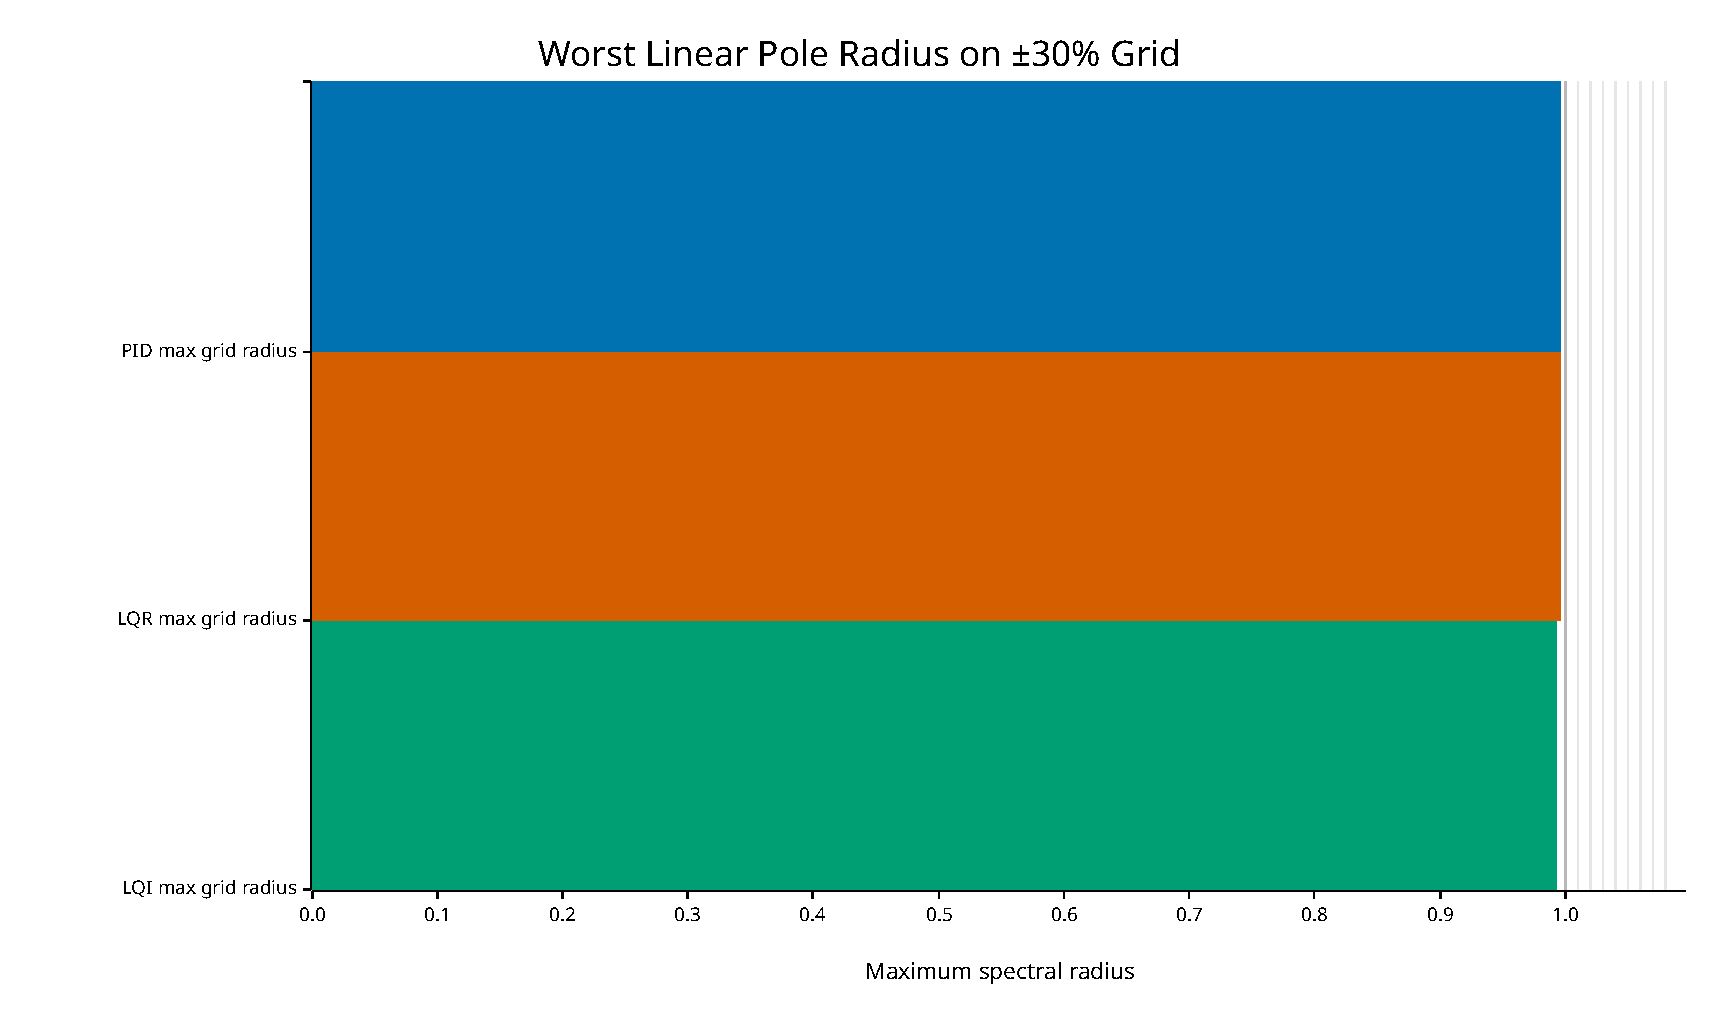
\includegraphics[width=\linewidth]{figures/stability-domain-summary.pdf}\caption{정수 불확실성 격자에서의 최악 스펙트럼 반경. 구간 증명이 아니라 보조 수치 근거이다.}\label{fig:stability}\end{figure}
\FloatBarrier
